\chapter{Semi-Automatic Annotation} \label{chapter:semi_automatic}

\begin{figure}[!tbp]
	\centering
    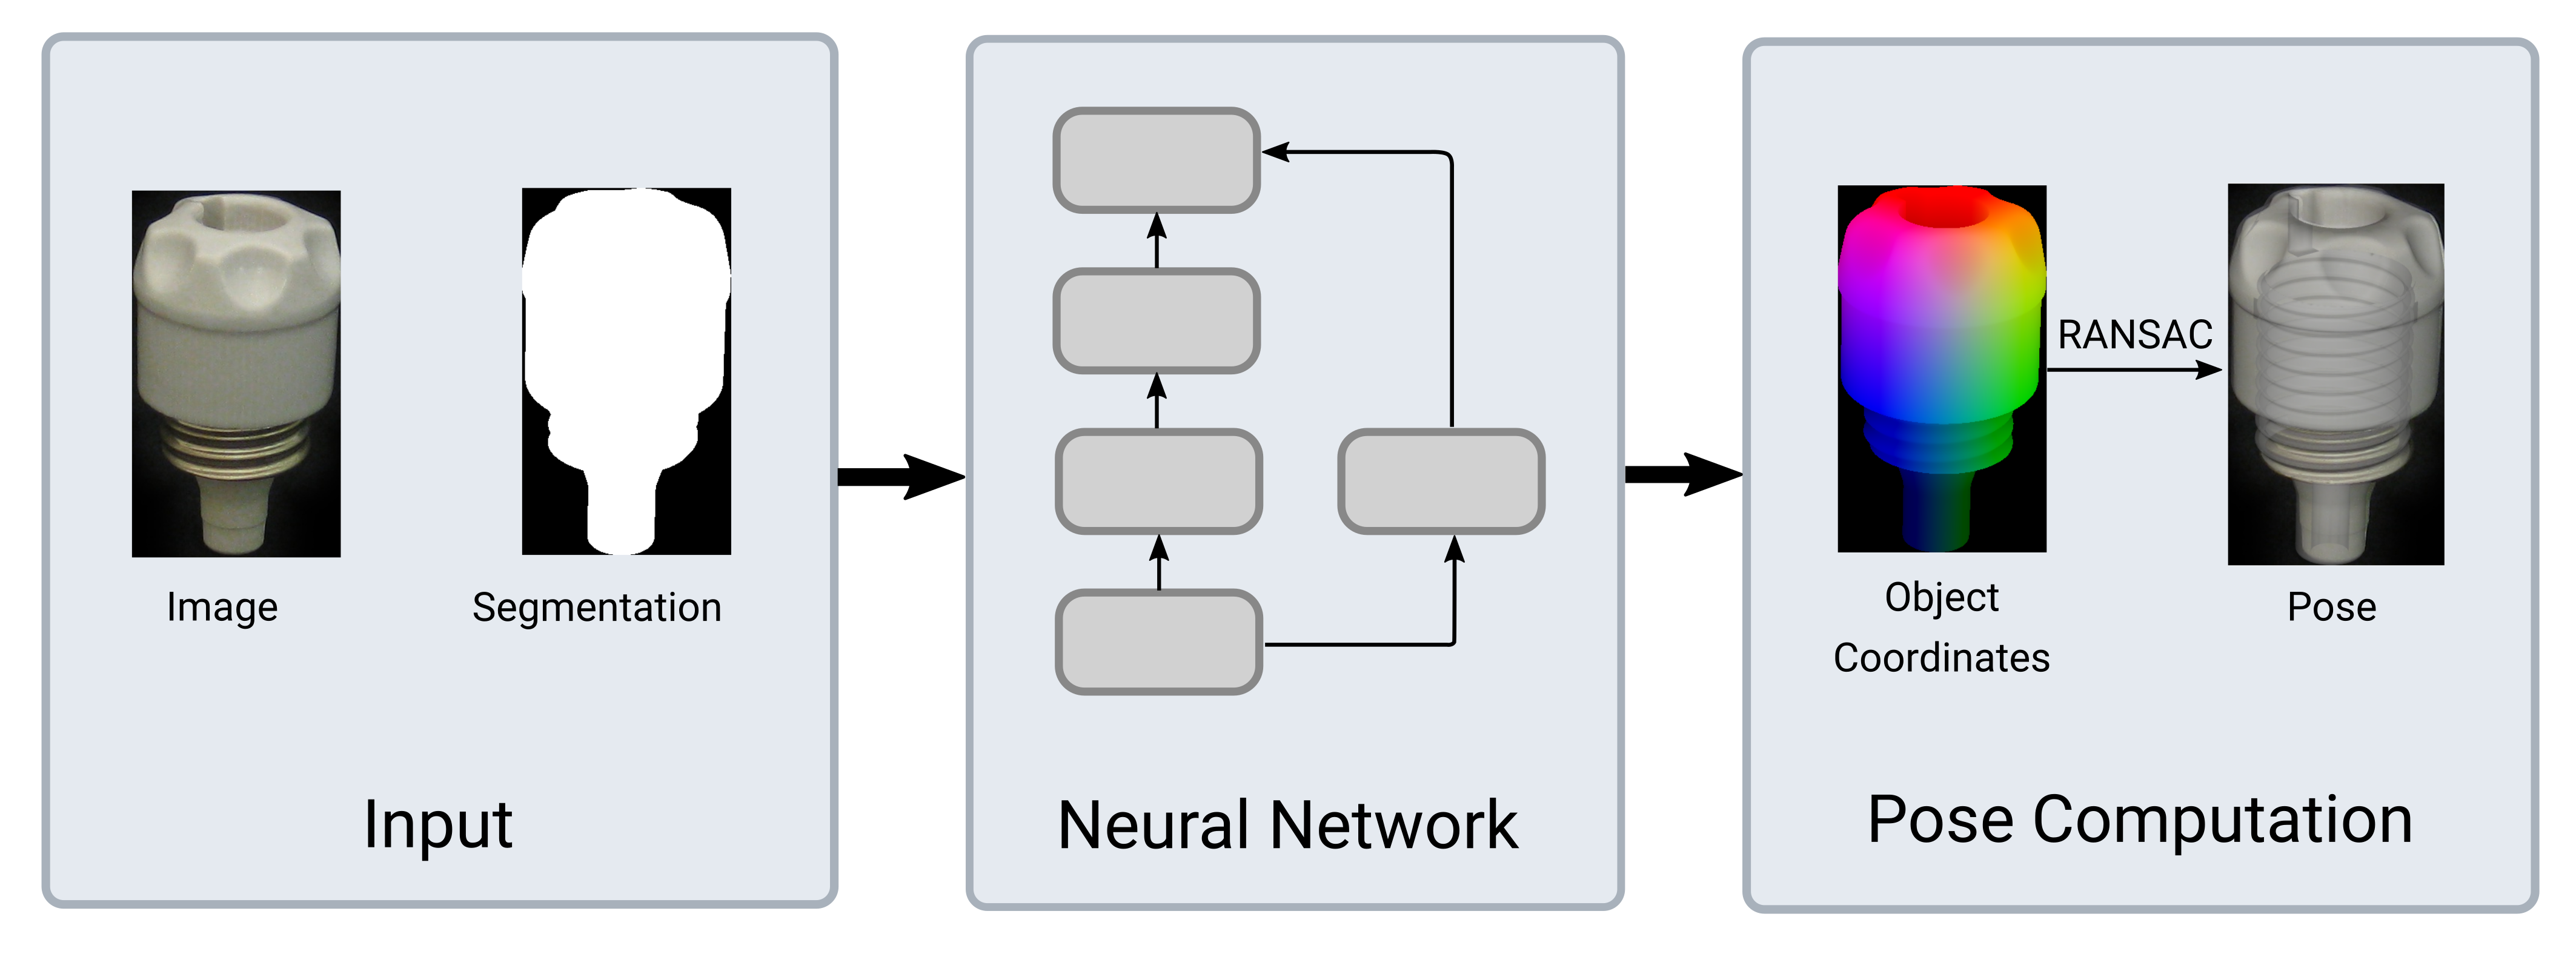
\includegraphics[width=\linewidth]{network_pipeline}
    \caption{The pipeline of the neural network. The two inputs of the network are the image and the corresponding segmentation image. The neural network then uses the segmentation to retrieve the pixels to predict object coordinates for. In the final pose computation stage the object coordinates and their 2D locations are used to retrieve the best pose using RANSAC.}
    	\label{fig:network_pipeline}
\end{figure} 

To assist in the process of manual image annotation presented in Chapter \ref{chapter:manual_annotation}, we developed a neural network for the task of 6D pose estimation tailored to the characteristics of the images of the Endoscopic Vision Challenge. This chapter describes the network architecture and its variations, as well as different approaches to train the network and the resulting modified annotation procedure.

\section{Terminology} \label{section:network_terminology}

\noindent\textbf{Residual Connection.} A \textit{residual connection} (or \textit{skip connection}) is a part of a neural network that skips some layers of the network and adds the input of a layer to the output of a layer that is situated deeper in the network. They can prevent the problem of the increasing training error in deeper networks \cite{resnet}. Fig. \ref{fig:residual_connection} visualizes such a connection. \\

\noindent\textbf{Training Set.} A \textit{training set} is a subset of the dataset intended to train a neural network with. The network uses the training set to adjust its weights as opposed to the validation set. \\

\noindent\textbf{Training Example.} A \textit{training example} is an element from the training set fed to the neural network during training. \\

\noindent\textbf{Training Batch.} A \textit{training batch} consists of a subset of training examples. During training the network updates its weights using all examples in the batch. \\

\noindent\textbf{Validation Set.} A \textit{validation set} is a subset of the dataset intended to train a neural network with. The validation set's purpose is to validate the network's new configuration which emerged from a run within the training. \\

\noindent\textbf{L1 Loss.} The \textit{L1 loss} is a loss function that sums up the results of the function $g$ applied to the $k$ elements in a training batch, i.e. $L_1(x, y) = \frac{1}{k} \sum\limits_k |g(x_k, y_k)|$. We set $g$ to be the euclidean distance: $g(x_k, y_k) = \sqrt{\sum\limits_i (x_{ki} - y_{ki})^2}$, $x_{ki}$ and $y_{ki}$ being the $i$-th entries of the vectors $x_k$ and $y_k$. \\

\noindent\textbf{L2 Loss.} The \textit{L2 loss} is a loss function defined similarly to the L1 loss but sums up the squared instead of the absolute results of $g$, i.e. $L_2(x, y) = \frac{1}{k} \sum\limits_k g(x_k, y_k)^2$. \\

\noindent\textbf{L2 Regularization.} \textit{L2 regularization} penalizes the weights by a factor $\lambda$ in the following way: $\lambda \sum\limits_i w_i^2$. The regularization term is added to the weight update to keep the network from overfitting. \\

\noindent\textbf{Dropout Percentage.} \textit{Dropout percentage} is the percentage of neurons to deactivate in a layer during training. \\

\noindent\textbf{Receptive Field-Size.} The \textit{receptive field-size} of a network denotes how many input pixels an output value of the network has taken into account. This factor is determined by the number of operations in the network and their parameters. A convolution operation can skip pixels, which results in a larger receptive field-size. Increasing the kernel size has the same effect. Depending on the field of application a field-size should be larger or smaller.

\section{Implementation}

The neural network and all of its functionality is implemented in Python using Tensorflow \cite{tensorflow} and Keras \cite{keras}. Tensorflow is a deep-learning framework that uses C++ to perform the actual calculations. It provides many different types of network layers, as well as tools to modify images, automatic differentiation of the loss function and optimization algorithms. Keras is a framework that makes using Tensorflow easier and allows to create neural networks in a few lines of code. Most of the operations of Tensorflow and Keras are performed in C++ but both can be easily used from Python. Both fromeworks offer functionality to transfer the computations to the graphics cards. This allows training deep networks in a feasible time \cite{ylecun}.

\begin{figure}[!tbp]
	\centering
	\begin{subfigure}[t]{0.47\textwidth}
		\centering
    	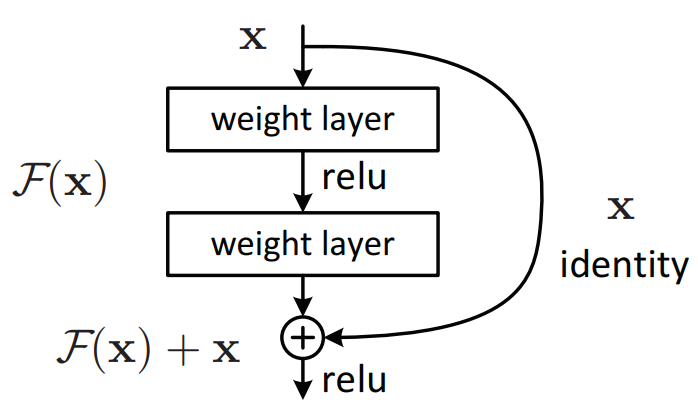
\includegraphics[width=\linewidth]{residual_connection}
    	\caption{A detailed view on a residual connection. The residual connections add the input of earlier layers of the network to deeper ones.}
    	\label{fig:residual_connection}
	\end{subfigure}
	\hfill
	\begin{subfigure}[t]{0.47\textwidth}
		\centering
    	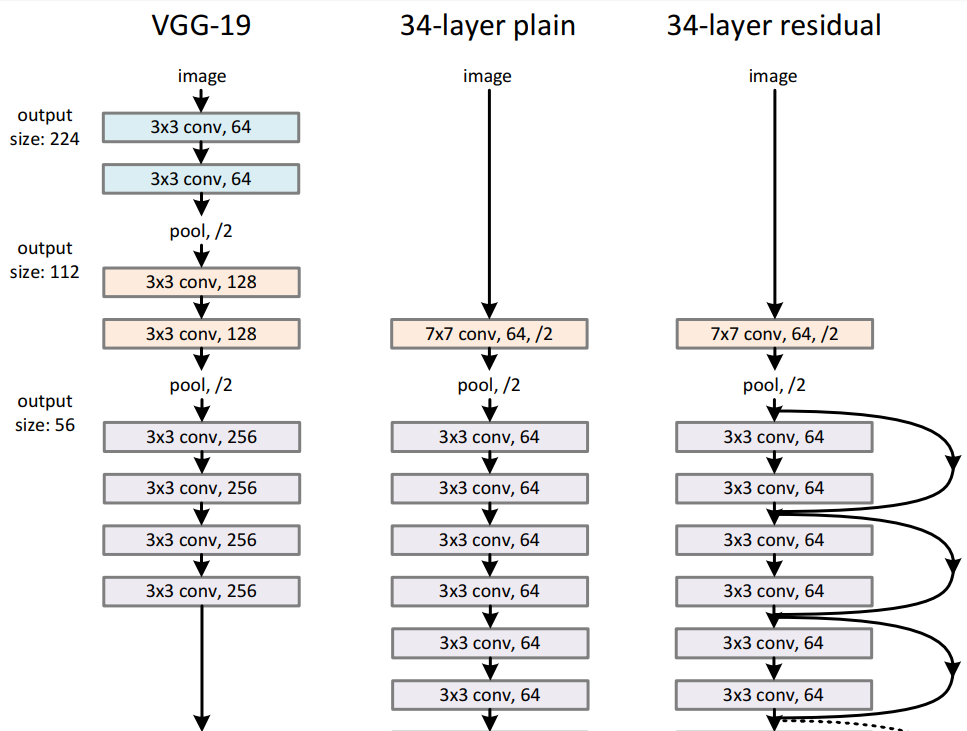
\includegraphics[width=\linewidth]{resnet_comparison}
    	\caption{Excerpt of a comparison between the ResNet architecture and VGG. ResNet allows the creation of deeper network, as the problem of vanishing gradients can be targeted this way. The image has been cropped.}
    	\label{fig:resnet_comparison}
	\end{subfigure}
	\caption{A key component of ResNet: the residual connection. The left image shows the connection in detail and the right image shows a comparison with the VGG architecture. Images from \cite{resnet}.}
	\label{fig:resnet_details}
\end{figure} 

\section{Network Architecture}

%TODO re-read

The architecture of the network is adjusted to the problem domain of the images of the Endoscopic Vision Challenge. There is no mechanism of inferring the masks and the network expects RGB-only images without depth information. This significantly reduces the complexity of predicting the position of the object. Heavily contradicting object coordinates can still lead to positional errors, though. \fig \ref{fig:network_pipeline} shows the processing pipeline of the network which takes the image and the segmentation image as inputs. The network processes each pixel which is part of the object according to the segmentation image and outputs the 3D coordinates. As explained in Chapter \ref{chapter:background}, we then compute the optimal pose using RANSAC and the 2D-3D correspondences.

The basic architecture that we chose for the network is called ResNet. He \etal first presented ResNet in 2015, which enabled researchers to create deeper networks than before \cite{resnet}. Two major problems arise in very deep neural networks. One is the vanishing gradients problem, which means that gradients gradually become 0 in deeper layers. A 0 gradient implies that the weights won't be changed. This problem can be targeted with batch normalization. The scond problem is that making a network deeper without further adjustments can lead to an increasing training eror. Adding layers to a network to increase expressivity does not directly lead to a higher accuracy. Even stacking identity layers, i.e. layers that learn the mathmatical identity function $f(x) = x$, ontop of the network increases the training error. This phenomenom can be partly compensated with residual connections \cite{resnet}. An example of a residual connection can be seen in \fig \ref{fig:residual_connection}. Fig. \ref{fig:resnet_comparison} shows a comparison of ResNet with the architecture \textit{VGG} \cite{vgg}. The residual connections are clearly visible as the arcs of the rightmost architecture.

We chose ResNet over other architectures due to its easy scalability and its still superior performance in terms of accuracy. Mask RCNN is a prominent example that makes use of ResNet's structure \cite{mask_rcnn}. The Facebook AI Research team developed Mask RCNN. The network is still ranking within the top 5 networks of the MS COCO challenge, as of July 2018. The MS COCO challenge is a challenge on image segmentation and object detection \cite{mscoco}.

The structure of the network is visualized in \fig \ref{fig:network_architecture}. The depicted architecture has 23 convolutional layers. The building blocks of the network are the \textit{Conv Block} and the \textit{ID Block}. Both blocks are shown in detail on the right. A Conv Block applies another convolution to the shortcut connection on the right and then combines the result with the output of the left path. The ID Block simply adds the input to the result of the convolutions on the left. The figure doesn't show the batch normalization and \textit{activation layers} to keep the illustration clear. The actual network has a batch normalization layer after each convolution layer and an activation layer after each batch normalization layer. Activation layers are layers in Keras that apply a specified activation function to their input. This way, non-linear neurons are realized in the framework.

\subsection{Loss Function \& Optimizer}

%TODO re-read

Since the network outputs the 3D coordinates for each pixel in the input image a straight-forward approach is to penalize the euclidean distance with respect to the ground-truth coordinates. The loss function sums up the absolute distances of the individual XYZ components of the predicted object coordinate and the ground-truth, but only at the relevant positions according to the segmentation mask. This resembles the L1 loss (see Section \ref{section:network_terminology}). The reason why we chose the L1 loss over the L2 loss is that the L2 loss penalizes outliers more. Outliers will already get eliminated in the RANSAC algorithm during pose computation. The L2 loss might strive for a worse compromise. We used L2 regularization for the weights. We compared SGD and Adam to find the best optimizer for the network (see Chapter \ref{chapter:background} for details on the optimizers).

\begin{figure}[!tbp]
	\centering
    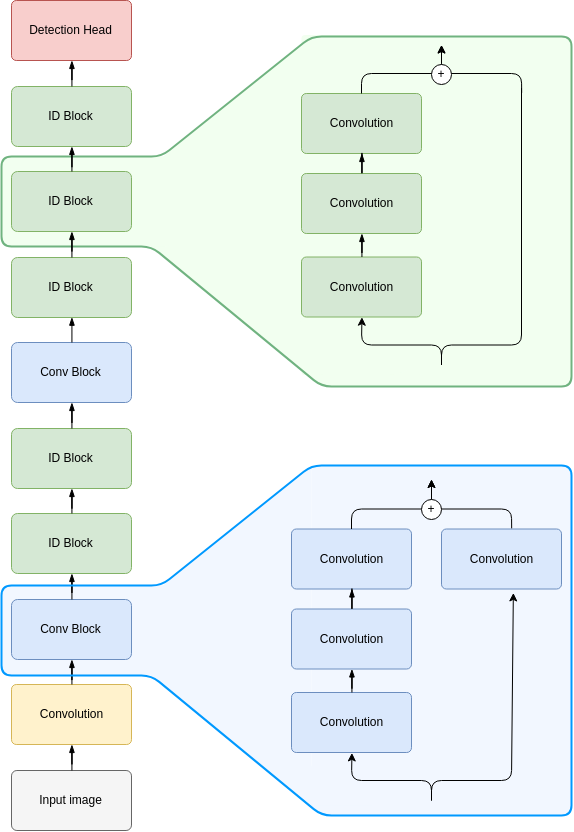
\includegraphics[width=0.9\linewidth]{flowerpower_short}
    \caption{Architecture 1 with a total of 23 (convolutional) layers. The components of the \textbf{Conv Block} and \textbf{ID Block} elements are visualized on the right. The characteristic of the Conv Block is that it applies a convolution on the shortcut connection while the ID Block doesn't. The yellow \textbf{Convolution} rectangle is a plain convolution layer. The \textbf{Network Head} consists of another three convolution layers.}
    	\label{fig:network_architecture}
\end{figure}

\subsection{Variations} \label{section:network_variations}

%TODO re-read

\begin{table}[]
\centering
\begin{tabular}{|l||llllll|}
\hline Architecture No.        & 1          & 2          & 3          & 4          & 5          & 6        \\ \hline\hline
\rowcolor{Gray}
\# Layers               & 23         & 35         & 23         & 50         & 50         & 50       \\
Receptive field-size    & 99         & 67         & 51         & 59         & 59         & 59       \\
\rowcolor{Gray}
\# Parameters & 3,95  & 19,69 & 6,32  & 24,63 & 24,63   & 24,63 \\
Data normalization      & bn & bn & bn & do    & bn & do \\ \hline
\end{tabular}
\caption{Overview over the differences between the network architectures. The number of layers corresponds to the number of convolutional layers. Batch normalization layers are not counted. The abbreviations \textit{bn} and \textit{do} stand for batch normalization and dropout, respectively. The number of parameters is given in millions. The number of parameters resembles the number of trainable variables in the network.}
\label{table:network_architectures}
\end{table}

To find the optimal network structure a total of 6 network architectures were created and later compared in Chapter \ref{chapter:experiments}. The first design of the network consisted of 23 convolutional layers with a receptive field-size of 99. A characteristic of the Endoscopic Vision Challenge dataset is that the tools have writings on them which is often not or only partly visible. To keep the network from detecting poses mainly based on the letters, we reduced the receptive field-size for the following architectures. We enlarged the second architecture to a total of 35 layers, while decreasing the receptive field-size to 67. The third architecture has the same number of layers like the first architecture but a reduced receptive field-size of 51. Architectures 4 to 6 all have a receptive field-size of 59 and the 50 convolutional layers. While architecture 5 uses batch normalization for regularization, the architectures 4 and 5 use dropout instead. The difference between those two is the dropout percentage. An overview over the architectures can be seen in Table \ref{table:network_architectures}. 

The number of parameters does not scale linearly with the number of layers, as deeper layers have more filters in the network. The reason why architecture 3 has more trainable parameters than architecture 1 is not entirely clear. The difference between the two networks is that architecture 3 uses a reduced kernel size on deeper layers to obtain a smaller receptive field-size. But this should not cause the number of parameters to grow in a fashion that is visible in the table.

%TODO reformulate
The reason why such diverse architectures were compared is that a focus of this work is to provide a prediction system that already produces satisfactory results with few images. A network with a higher number of trainable parameters can take longer to learn the training data and might overfit to it. A shallower network might produce worse results after the first training, but subsequently offer a better accuracy  as soon as more data is available.

%TODO refernce appendix

The different depths of the network architectures are visualized in appendix \ref{appendix:network_architectures}. The architectures that omit the batch normalization layers and employ dropout layers instead are not listed separately, because the depth of the convolutional layers is the same as in architecture 5.

\section{Setup}

Before the user can run the network to train on a dataset, some steps to setup the network have to be undertaken. Depending on the format of the file that holds the ground-truth poses of the images of the dataset, a conversion to the format expected by the network needs to be performed. An example conversion function is provided, which converts the T-Less format to the JSON format that the network is able to read. The T-Less dataset does not provide segmentation masks, nor object coordinates. The mask and coordinate images can be rendered using the images, the ground-truth poses file and the utility scripts of the network. After obtaining all the necessary data for training, the user needs to write a JSON configuration file, which holds the paths to the data and the parameters of the network. The network architecture that is to be trained can be named directly in the file. The network consists of convolutional, batch normalization and pooling layers only. This means it can be applied to arbitrary image sizes without having to retrain the network, as in contrast to networks employing fully-connected layers. If the image size changes, a fully-connected layer has to be retrained. The maximum image size needs to be specified in the configuration file, nevertheless. This is necessary, because the network is trained in batches instead of single training examples. Keras expects the samples to all have the same dimension. The size in the file can be simply increased if the user wants to run inference on larger images.

\section{Modes of Operation} \label{section:modes_of_operation}

\begin{figure}[!tbp]
	\centering
    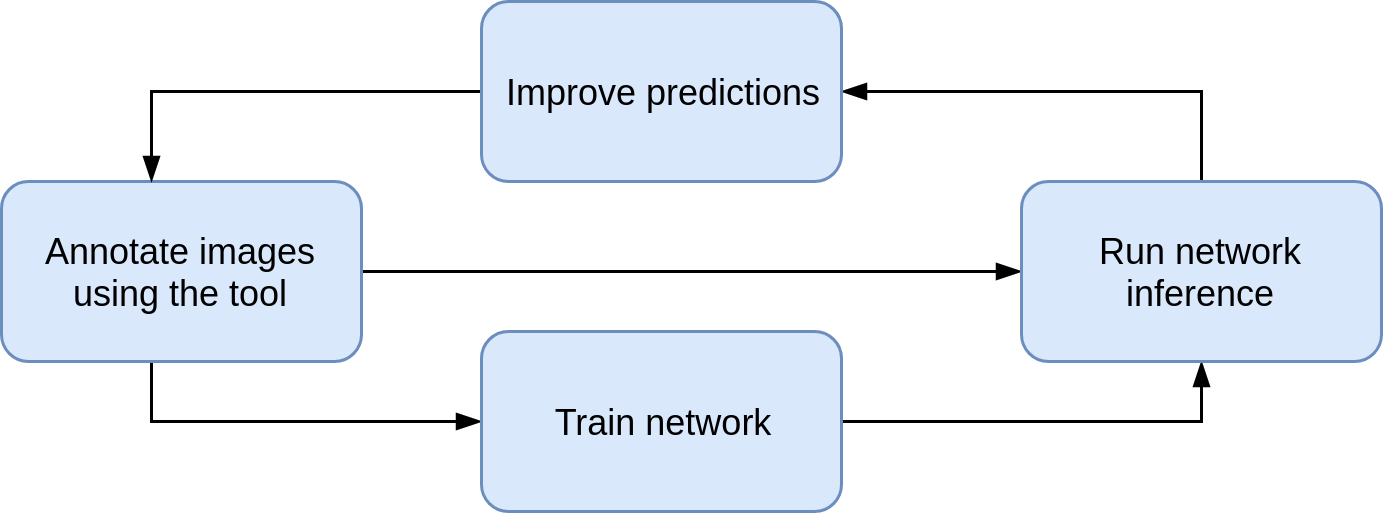
\includegraphics[width=0.75\linewidth]{semi_automatic_workflow}
    \caption{The new workflow of the annotation procedure including the neural network. First, the user has to annotate enough images from the dataset to be able to train the network. After successfully training the network it can be used to predict poses on a subset of the dataset. The user can then improve the poses and return to annotating more images or run the network inference on more images.}
    	\label{fig:semi_automatic_workflow}
\end{figure}

The goal of the neural network is to make the annotation process presented in chapter \ref{chapter:manual_annotation} faster and more efficient. To achieve this we strove for a symbiosis between the annotation tool and the neural network. The new workflow is visualized in \fig \ref{fig:semi_automatic_workflow}. In addition to manually annotating images, the user can train the network with the annotated data. After training the neural network can be used to predict predict poses in unseen images. As the network will likely make errors, the poses can be corrected afterwards using 6D-PAT. The improved pose predictions can serve as input to further train the network. A characteristic of the Endoscopic Vision Challenge dataset is that there aren't existing any annotated poses. Training the network is thus not as straightforward compared to a fully annotated dataset. The following sections describe different approaches of training the network, which are evaluated in Chapter \ref{chapter:experiments}.

%TODO rewrite

\subsection{Online Learning}

During the annotation process, the user can train the network using the new data. One option is to fully retrain the network with all  annotated images. This procedure is called \textit{training from scratch}. Another option is to train the network incrementally, instead. \textit{Incremental training} means that the user trains the network using the only the annotations added after the last training run. In this approach, the weights of the network are not initialized to 0 or randomly (only for the first run), but the weights of the last training run are loaded and trained further using the newly available data. Because the weights are already set meaningful values, this method is likely to converge faster. The next chapter experimentally compares those approaches.

\subsection{Active Learning}

To help the user decide which images annotate, a procedure can propose images for annotation. The proposals should be based on inaccurate predictions of the network. Correcting these predictions can help the network to improve its accuracy. This method requires a measure of the accuracy of the predicted poses. We provide an example measure in the next chapter.

%TODO check if the sentence "we provide a measure in the next chapter" is still correct in the end